\documentclass{beamer}
\usepackage{graphicx}
\usepackage{hyperref}
\usetheme{Boadilla}
\title{Sharpe Ratio Optimization Via Stochastic Gradient Descent}
\subtitle{Theory \& Implementation}
\author{Joe Nunez}
\institute{Harvey Mudd College}
\date{Feb. 28, 2018}

\begin{document}
\begin{frame}
\titlepage
\end{frame}

\begin{frame}
\frametitle{Previous Work}
My project is inspired by the thesis ``Geometry and Optimization of Relative Arbitrage'' by Ting-Kam Leonard Wong, which focuses on how geometric methods can be used to determine how market portfolio growth may be improved by through periodic rebalancing.
\vspace{.1in}
\\While this is not the main topic of my project, it provided a jumping-off point as I realized that stock market portfolios may be studied using information geometry.  I also use conclusions drawn from Shun-Ichi Amari's work on information geometry.
\end{frame}

%\begin{frame}
%\frametitle{Assumptions}
%\begin{enumerate}
%\item Discrete time
%\item 
%\end{enumerate}
%\end{frame}

\begin{frame}
\frametitle{Portfolio}
A portfolio can be regarded as a set of assets $a_i$, each with proportion $\pi_i$ between 0 and 1 corresponding to the portion of the portfolio allocated to that asset, and where the sum of all $\pi_i$ is 1.  There is no upper bound on the number of assets theoretically in a portfolio.
\vspace{.1in}
\\Immediately, we can see that the set of possible portfolios is a subset of the Statistic Manifold, $S$, in that the set is infinite-dimensional and has elements summing to exactly 1.  This will allow us to apply methods from information geometry to the analysis of portfolios.
\end{frame}

\begin{frame}
\frametitle{Information Geometry}
The Statistic Manifold $S$ is the set of all probability distributions.
\\When $S$ is restricted to $n$ dimensions, it creates an $n$-dimensional simplex. 
\begin{figure}[t]
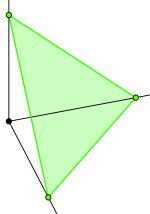
\includegraphics[scale=0.4]{simplex}
\centering
\end{figure}
As you can see when $n=3$, simplexes are quite flat (dually flat, as proved by Amari), which conveys a number of favorable properties.  Most notably, for the purposes of this project, $S$ is dually flat under $KL$-divergence, so a neural network performing stochastic gradient descent is guaranteed to converge to a global minimum. (Amari et al)
\end{frame}

\begin{frame}
\frametitle{Information Geometry}
In fact, the set of portfolios is isometric to the restriction of $S$ to finite dimensions.  It's actually very easy to prove.  Consider the map
\[(\pi_1, \dots, \pi_n) \rightarrow (\pi_1, \dots, \pi_n)\]
This map is clearly isometric under every metric since it is just the identity map.  Thus the set of portfolios is a differentiable, dually flat manifold, and all conclusions about $S$ for finite-dimensional distributions still hold.
\end{frame}

\begin{frame}
\frametitle{Basic Portfolio Theory}
Consider the returns $R_i$ of assets to be random variables (they have been empirically found to resemble a log normal distribution.  The risks $\sigma_i$ of assets can be represented as the standard deviation in the returns, and the rates of return $r_i$ can be represented with mean returns (typically found using daily log continuous growth rates for the past year or two).  (Wong)
\end{frame}

\begin{frame}
\frametitle{Portfolio Returns}
For a portfolio of $n$ assets with portfolio weights $\pi_1, \pi_2, \dots, \pi_n$ and return rates $r_1, r_2, \dots, r_n$, the return of the portfolio overall is 
\[r_P = \pi_1r_1 +\pi_2r_2 + \dots + \pi_n r_n = \sum_{i=1}^n \pi_i r_i\]
(Wong)
\end{frame}

\begin{frame}
\frametitle{Portfolio Risk}
Financial assets often have correlated performance, so it is important to account for this when estimating the risk level in a portfolio.  The variance of the returns for a portfolio with non-independent assets is calculated as
\[\sigma^2_P = \sum_{i,j=1}^n \pi_i \pi_j \text{Cov} (R_i, R_j),\]
where $\text{Cov} (R_i, R_j)$ is the covariance of the returns for assets $i$ and $j$.  (Wong)
\end{frame}

\begin{frame}
\frametitle{Manifold of Returns}
Notice that for any portfolio $P$, that portfolio has an expected rate of return $r_P$ and risk level $\sigma_P$.  Therefore, each portfolio can be mapped to a probability distribution.

Interestingly, this family of distributions is also in $S$, though a different family: the family of normal distributions.  Fortunately, we have a very good metric for measuring distances between normal distributions: the Kullback-Leibler Divergence, which calculates the distance between distributions as the amount of non-overlapping area under the curves.
\end{frame}

\begin{frame}
\frametitle{Portfolio Theory Problems}
A common goal of investors is to get the highest possible return with the lowest possible risk.  To evaluate an investment strategy using this criteria, investors consider the Sharpe ratio.
The Sharpe ratio is the rate of return over the risk level of an investment, so for a portfolio, the Sharpe ratio is
\[\frac{r_P}{\sigma_P},\]
Therefore, the problem is to maximize this ratio.
\end{frame}

\begin{frame}
\frametitle{Convex Optimization Problems}
I should note that one approach that the Wong paper uses is to represent the optimization problem as a convex constraint optimization problem and leverage approaches from convexity.

This approach is computationally difficult, (and less related to this course), but it is worth mentioning as a solution to the problem.
\end{frame}

\begin{frame}
\frametitle{Sharpe Ratio Maximization}
A neural network seeks to minimize the distance between predictions and targets for a dataset according to a particular loss function using stochastic gradient descent. 
\vspace{.1in}
\\We will use an adaline, a neural network with only an input and output layer, to determine the optimal portfolio weights for a given set of assets.  To do so, we'll use the $KL$-divergence as a loss function, and make the target be a normal distribution with an unachievably high rate of return and low risk.  
\end{frame}

\begin{frame}
\frametitle{Sharpe Ratio Maximization}
The prediction our network produces will be the distribution corresponding to the portfolio with proportions corresponding to the connections weights (after normalized).
\vspace{.1in}
\\Once the network converges, the connection weights of the network will give the optimal portfolio configuration.
\end{frame}

\begin{frame}
\frametitle{Stochastic Gradient Descent}
The basic idea of stochastic gradient descent is to travel downward along the gradient of the error surface for a predictor.
\begin{figure}[t]
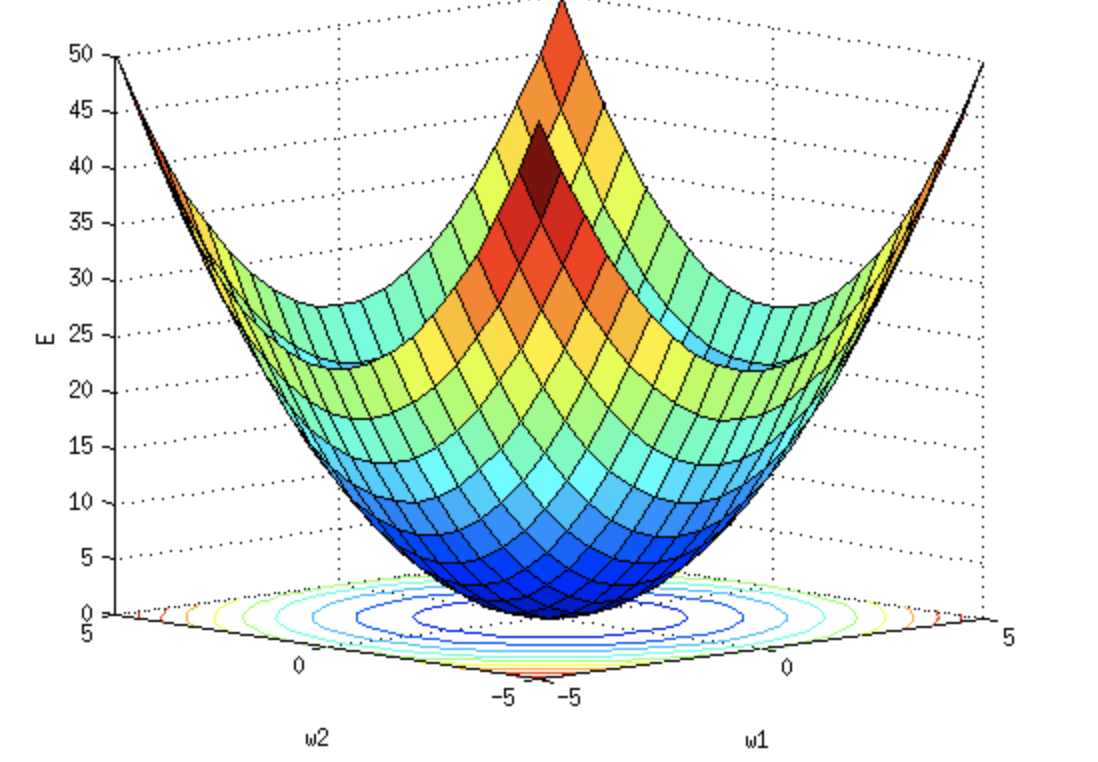
\includegraphics[scale=0.4]{errorsurface}
\centering
\end{figure}
To do so, we'll need to calculate the gradient for our portfolio: the rate of change of the error function with respect to the weights of each of our assets.
\end{frame}

\begin{frame}
\frametitle{Gradient of KL-Divergence}
For two normal distributions $p$ and $q$ with respective standard deviations $\sigma_1$ and $\sigma_2$ and means $\mu_1$ and $\mu_2$, the KL divergence is given by 
\[KL(p,q) = \log\frac{\sigma_2}{\sigma_1} + \frac{\sigma_1^2 + (\mu_1 - \mu_2)^2}{2\sigma_2^2} - \frac{1}{2}\]
Note that our target distribution is constant.  $\mu$ and $\sigma$ for our prediction, which we will say is $p$, are given by
\[\mu = \sum_{i=1}^n \pi_i r_i = \mu^T \pi = \pi^T \mu\]
\[\sigma = \sqrt{\sum_{i,j=1}^n \pi_i \pi_j \text{Cov} (R_i, R_j)} = \sqrt{\pi^T C\pi}\]
Note also that the covariances and rates of returns for the assets are constants.
\end{frame}

\begin{frame}
\frametitle{Gradient of KL-Divergence (Cont.)}
Now let us calculate $\frac{\partial KL(p,q)}{\partial \pi_i}$.  We can do so for a generic $i$ as each appears in a similar form in the summations.  First, we plug in our expressions for $\sigma_1$ and $\mu_1$:
\[KL(p,q) = \ln \sigma_2 - \frac{1}{2}\ln (\pi^T C \pi) \]\[ + \frac{1}{2\sigma_2^2}[\pi^TC\pi+ (\mu^T\pi- \mu_2)^2] - \frac{1}{2}\]

%\[KL(p,q) = \ln \sigma_2 - \ln \sqrt{\sum_{i,j=1}^n \pi_i \pi_j \text{Cov} (R_i, R_j)} \]\[ + \frac{\sum_{i,j=1}^n \pi_i %\pi_j \text{Cov} (R_i, R_j) + (\sum_{j=1}^n \pi_j r_j - \mu_2)^2}{2\sigma_2^2} - \frac{1}{2}\]
\end{frame}

\begin{frame}
\frametitle{Gradient of KL-Divergence (Cont.)}
Now let us calculate $\frac{\partial KL(p,q)}{\partial \pi_i}$.  We can do so for a generic $i$ as each appears in a similar form in the summations.
\[\nabla_\pi KL(p,q) = -\frac{1}{2 \pi^T C\pi} ( 2 C\pi ) + \frac{1}{2\sigma_2^2}[2 C\pi +2(\pi^T\mu- \mu_2)\mu] \]
Or
\[\frac{\partial KL(p,q)}{\partial \pi_i} =  - \frac{\sum_{j=1, j\neq i}^n \pi_j \text{Cov} (R_i, R_j)}{2\sum_{i,j=1}^n \pi_i \pi_j \text{Cov} (R_i, R_j)} \]
\[ + \frac{\sum_{j=1, j \neq i}^n \pi_j \text{Cov} (R_i, R_j)}{2\sigma_2^2} + \frac{r_i (\sum_{j=1}^n \pi_j r_j - \mu_2)}{\sigma_2^2} \]
\[- \frac{ \pi_i}{\sum_{i,j=1}^n \pi_i \pi_j \text{Cov} (R_i, R_j)} + \frac{\pi_i}{\sigma_2^2} \]
Note that the third line terms come from there being a $\pi_i^2$ term in the summations for $\sigma_1^2$
\end{frame}


\begin{frame}
\frametitle{Results}
I implemented a stochastic gradient descent algorithm using this function and data from quandl for a number of heavily traded stocks.

The daily Sharpe ratio that my algorithm converged at was 
\[\frac{1.00092837293}{1.00696895367} = 0.994001224448\]
which I checked against the Sharpe ratios for each of the individual assets and found that exceeded each of the individual ratios.
\end{frame}

\begin{frame}
\frametitle{Results (Cont.)}
The algorithm converged on a set of weights which had a daily rate of log return of 0.09\%, which compounds to a yearly rate of growth of 26.3\%.
The portfolio had a standard deviation of yearly returns of 11.6\%, indicating that the event of our portfolio losing money has a $z$-score (in terms of a normal distribution) of $-2.46$, indicating that our portfolio's chance of losing money is less than 1\% according to this measure of risk.
\vspace{.1in}
\\Additionally, I ran the gradient descent algorithm multiple times and always converged to the exact same loss (up to the maximum float precision), indicating empirically that the solution was indeed the global optimum.
\end{frame}

\begin{frame}
\frametitle{Opportunities for Expansion}
Wong's thesis actually focuses on volatility harvesting, the theory of which goes as follows:

Since riskier assets tend to grow faster than safer ones, a portfolio tends to get riskier as it grows, and therefore requires rebalancing.  As a result, we want portfolios to be safer than our risk tolerance immediately after we rebalance, then wait to rebalance until the risk level exceeds our threshold, and rebalance at such a time that the average risk over the time period between rebalancing is at our threshold.  Creating an algorithm for determining what risk levels and portfolio configurations should be rebalanced to and from to optimize growth is a plausible extension for this project.
\end{frame}

\begin{frame}
\frametitle{Sources}
Wong, T. 2016, 'Geometry and Optimization of Relative Arbitrage', PhD Thesis, University of Michigan, Ann Arbor MI.
\url{http://ieeexplore.ieee.org/stamp/stamp.jsp?arnumber=125867}
\\\url{https://stats.stackexchange.com/questions/7440/kl-divergence-between-two-univariate-gaussians}
\\\url{https://www.pyimagesearch.com/2016/10/17/stochastic-gradient-descent-sgd-with-python/}
\\\url{https://docs.scipy.org/doc/numpy/reference/}
\\\textbf{Data}
\\\url{https://www.quandl.com/}
\\\textbf{Images}:
\\\url{https://en.wikipedia.org/wiki/Simplex}
\\\url{https://commons.wikimedia.org/wiki/File:Error_surface_of_a_linear_neuron_with_two_input_weights.png}
\end{frame}

\end{document}
